\documentclass[a4paper]{article}

\usepackage[english]{babel}
\usepackage{amsmath}
\usepackage{amsfonts}
\usepackage{amssymb}
\usepackage{graphicx}
\usepackage{hyperref}
\hypersetup{hidelinks}
\usepackage{amsthm}

\newtheorem{theorem}{Theorem}
\newtheorem{lemma}{Lemma}

\begin{document}
\pagenumbering{arabic}

\begin{center}
{\Large Error in Euler's Method\\}

\vspace{10pt}

{\large Julio A. Medina$^1$\\}
\vspace{10pt}
{\small
$^1$ Universidad de San Carlos de Guatemala\\
School of Physical and Mathematical Sciences\\
Master's Program in Physics\\
\href{mailto:julioantonio.medina@gmail.com}{julioantonio.medina@gmail.com}\\
}
\end{center}

\vspace{10pt}

\section{Euler's Method}

Euler's method is the most elementary technique for approximating the solution of an initial value problem. Although its practical use is limited, the simplicity of its derivation makes it useful for illustrating and guiding the construction of more elaborate numerical techniques without first having to deal with their more involved algebra.

The objective of Euler's method is to obtain an approximation to the well-posed initial value problem

\begin{equation}\label{prob1}
\frac{dy}{dt}=f(t,y), \qquad a\leq t\leq b, \qquad y(a)=\alpha.
\end{equation}

The result produced by Euler's method is not a continuous approximation. Instead, it consists of approximate values at selected locations, known as mesh points, in the interval $[a,b]$. Once approximations at the mesh points have been obtained, intermediate values can be estimated using an interpolation technique.

First, all mesh points are chosen to be equally spaced in $[a,b]$. This condition is imposed by selecting a positive integer $N$ and defining

\begin{equation*}
t_i=a+ih, \qquad i=0,1,2,\ldots,N.
\end{equation*}

The common distance between consecutive mesh points,

\begin{equation*}
h=\frac{b-a}{N}=t_{i+1}-t_i,
\end{equation*}

is called the step size. Euler's method can be derived from a Taylor expansion. Suppose that $y(t)$, the unique solution of Problem~\ref{prob1}, has two continuous derivatives on $[a,b]$. Then, for each $i=0,1,2,\ldots,N-1$,

\begin{equation*}
y(t_{i+1})=y(t_i)+(t_{i+1}-t_i)y'(t_i)+\frac{(t_{i+1}-t_i)^2}{2}y''(\xi_i),
\end{equation*}

for some $\xi_i\in(t_i,t_{i+1})$. Using $h=t_{i+1}-t_i$ gives

\begin{equation*}
y(t_{i+1})=y(t_i)+hy'(t_i)+\frac{h^2}{2}y''(\xi_i).
\end{equation*}

Because $y(t)$ satisfies the differential equation in Problem~\ref{prob1},

\begin{equation}\label{euler_method1}
y(t_{i+1})=y(t_i)+hf(t_i,y(t_i))+\frac{h^2}{2}y''(\xi_i).
\end{equation}

Euler's method approximates $y(t_i)$ by $w_i$ and omits the last term in Equation~\ref{euler_method1}. Therefore, the method is defined by

\begin{equation}
\begin{split}
w_0&=\alpha,\\
w_{i+1}&=w_i+hf(t_i,w_i), \qquad i=0,1,\ldots,N-1.
\end{split}
\end{equation}

Euler's method was implemented in a Python script to analyze the behavior of its error. The source code is available at \url{https://github.com/Julio-Medina/Euler-Method/tree/main/python}.

\subsection{Error Behavior in Euler's Method}

To illustrate the error behavior of Euler's method, consider the initial value problem

\begin{equation*}
y'=y-t^2+1, \qquad 0\leq t\leq 2, \qquad y(0)=0.5.
\end{equation*}

The exact solution is

\begin{equation*}
y(t)=(t+1)^2-\frac{1}{2}e^t.
\end{equation*}

Using the Python script mentioned above produces the results shown in Figure~\ref{table}.

\begin{figure}[ht]
\centering
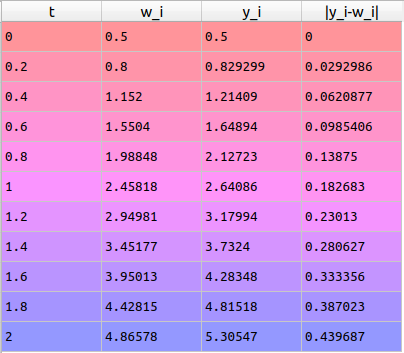
\includegraphics[scale=0.38]{../report/table1.png}
\caption{Numerical values used to analyze the error in Euler's method.}
\label{table}
\end{figure}

Figure~\ref{plot} shows the exact solution and its Euler approximation graphically.

\begin{figure}[ht]
\centering
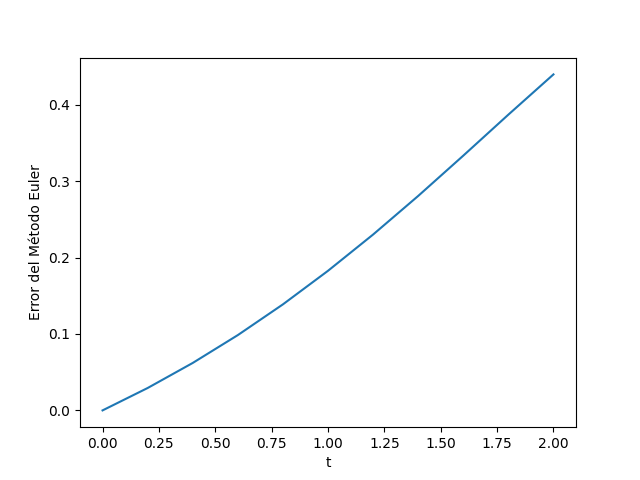
\includegraphics[scale=0.4]{../report/plot1.png}
\caption{Exact solution and Euler approximation.}
\label{plot}
\end{figure}

The pointwise error increases as $t$ increases. This controlled error growth is consistent with the stability assumptions used in the error analysis. More precisely, the theorem in the next section shows that the global discretization error is proportional to the step size $h$ over a fixed interval.

\section{Error Bounds for Euler's Method}

Although Euler's method is not sufficiently accurate for many practical applications, the error produced by the method is relatively easy to analyze. The error analyses of more accurate methods follow a similar pattern, although their derivations are more involved.

Two computational lemmas are useful for deriving an error bound for Euler's method.

\begin{lemma}\label{lemma1}
For every $x\geq -1$ and every positive integer $m$,

\begin{equation*}
0\leq (1+x)^m\leq e^{mx}.
\end{equation*}

\begin{proof}
Taylor's theorem applied to $f(x)=e^x$ about $x_0=0$ gives

\begin{equation*}
e^x=1+x+\frac{x^2}{2}e^{\xi}
\end{equation*}

for some $\xi$ between $0$ and $x$. Therefore, $1+x\leq e^x$. Since $x\geq -1$, we also have $1+x\geq 0$. Raising both sides to the positive integer power $m$ yields

\begin{equation*}
0\leq (1+x)^m\leq (e^x)^m=e^{mx}.
\end{equation*}
\end{proof}
\end{lemma}

\begin{lemma}\label{lemma2}
Let $s$ and $t$ be positive real numbers, and let $\{a_i\}_{i=0}^{k}$ be a sequence satisfying $a_0\geq -t/s$ and

\begin{equation}\label{ineq1}
a_{i+1}\leq (1+s)a_i+t, \qquad i=0,1,2,\ldots,k-1.
\end{equation}

Then

\begin{equation*}
a_{i+1}\leq e^{(i+1)s}\left(a_0+\frac{t}{s}\right)-\frac{t}{s}.
\end{equation*}

\begin{proof}
For a fixed integer $i$, repeated application of Inequality~\ref{ineq1} gives

\begin{equation}\label{eq:proof}
\begin{split}
a_{i+1}
&\leq (1+s)a_i+t\\
&\leq (1+s)[(1+s)a_{i-1}+t]+t\\
&=(1+s)^2a_{i-1}+[1+(1+s)]t\\
&\leq (1+s)^3a_{i-2}+[1+(1+s)+(1+s)^2]t\\
&\ \vdots\\
&\leq (1+s)^{i+1}a_0+[1+(1+s)+(1+s)^2+\cdots+(1+s)^i]t.
\end{split}
\end{equation}

The finite geometric series satisfies

\begin{equation*}
\sum_{j=0}^{i}(1+s)^j=\frac{(1+s)^{i+1}-1}{s}.
\end{equation*}

Substituting this result into Equation~\ref{eq:proof} gives

\begin{equation*}
a_{i+1}\leq (1+s)^{i+1}\left(a_0+\frac{t}{s}\right)-\frac{t}{s}.
\end{equation*}

Because $a_0+t/s\geq 0$, Lemma~\ref{lemma1}, applied with $x=s$, implies

\begin{equation*}
a_{i+1}\leq e^{(i+1)s}\left(a_0+\frac{t}{s}\right)-\frac{t}{s}.
\end{equation*}
\end{proof}
\end{lemma}

\begin{theorem}\label{euler-error-theorem}
Suppose that $f$ is continuous and satisfies a Lipschitz condition in the second variable with constant $L$ on

\begin{equation*}
D=\{(t,y)\mid a\leq t\leq b,\ -\infty<y<\infty\},
\end{equation*}

and suppose that a constant $M$ exists such that

\begin{equation*}
|y''(t)|\leq M, \qquad t\in[a,b],
\end{equation*}

where $y(t)$ is the unique solution of the initial value problem

\begin{equation*}
y'=f(t,y), \qquad a\leq t\leq b, \qquad y(a)=\alpha.
\end{equation*}

If $w_0,w_1,\ldots,w_N$ are the approximations generated by Euler's method for a positive integer $N$, then, for every $i=0,1,2,\ldots,N$,

\begin{equation}
|y(t_i)-w_i|\leq \frac{hM}{2L}\left[e^{L(t_i-a)}-1\right].
\end{equation}
\end{theorem}

A proof of Theorem~\ref{euler-error-theorem} can be found in Burden and Faires~\cite{Burden}.

\begin{thebibliography}{99}

\bibitem{Burden}
Richard L. Burden and J. Douglas Faires,
\textit{Numerical Analysis},
9th ed., Brooks/Cole, Cengage Learning,
ISBN 978-0-538-73351-9.

\end{thebibliography}

\end{document}
